\subsection{Silicon Strip Tracker\label{subsec:SiTracker}} 
In standard p-p collision operation, the tracker detector sends the full detector information to 430 Front-End Driver (FEDs). 
They apply common mode noise subtraction and strip zero-suppression. However, the common noise subtraction algorithm implemented in the Tracker FEDs firmware doesn't allow
compensation of the baseline distortion observed in the presence of Highly Ionizing Particles (HIP), with the consequent
potential loss of clusters associated with the affected readout chip. Due to the stringent requirements on tracking for
high multiplicity HI events, the cluster-finding inefficiency propagates directly to the track-finding inefficiency,
depending on the centrality of the collision.

The solution adopted up to now was to bypass the tracker zero-suppression implemented in the tracker FEDs and send the
full detector information to the DAQ/HLT. HI-specific common mode noise subtraction and zero-suppression algorithms were
implemented as HLT processes. However, this solution results in a heavy load on the links between the FEDs and the DAQ
and on the DAQ itself. The links are based on S-Link technology with a maximum speed of 200 MB/s. Some FEDs (connected
to sensors in which higher multiplicity is expected) have duplicate links, allowing a maximum of $\sim 400$ MB/s per
FED.  Considering that on the average fragment size is ~32 kB/event (VR10 version), the readout limit is at around 12 kHz. It has
already been demonstrated that the FED itself is designed to sustain up to 520 MB/s of throughput. The limitation is
then only coming from the links to the DAQ.

In agreement with the Tracker group, the only solution available to significantly increase the overall L1 rate is to
modify the FEDs firmware reducing the data output to DAQ. The possible solution envisaged were two:

\begin{enumerate}
\item Design a new zero suppression algorithm 
\item Create an hybrid format in which only the data of APVs with distorted baseline are sent to the DAQ in Virgin Raw mode 
\end{enumerate}

In sections \ref{subsubsec:DerFollower} and \ref{subsubsec:hybridtracker} a detailed description of the two solutions is presented including the preliminary studies performed. 
After evaluation, it was decided that solution (2) represents the most interesting in term of performances and feasibility. 

For completeness, we should also report that other possible strategies were studied/considered to increase the L1 rate
without modifying the tracker FED FW. However, they were rejected as being either too complicated to be implemented or
as underperforming. The two other solutions envisaged were either to increase the number of links between the tracker
FEDs and the DAQ or to reduce the data payload. The first solution appears to be too complicated, adding an extra $\sim
400$ links. Apart from the technical constraints, there would also not be enough time to install and commission the
links during the available shutdown time. The second solution is to reduce the data payload. A FED firmware version
implemented already in 2015 allows the reduction from 10 to 8 in the number of bits read out by each strip ADC. However,
this strategy would allow only a moderate increase of $\le 20 \%$ of the overall L1 rate at the cost of a reduction of
the detector resolution/sensitivity. 

\subsubsection{Derivative follower algorithm \label{subsubsec:DerFollower}}
In 2013 a specific HI zero-suppression algorithm designed for high multiplicity environments that would satisfy the FPGA
constraints was designed offline; it is named a ``Derivative Follower''. It scans the APVs and it finds gradients. A positive slope can represent the beginning of a cluster while a negative slope can represent the end of a cluster. Checks on the cluster shape are included in the algorithm. 

Implementing the algorithm in firmware would give the maximum data reduction to HLT having an average event size of roughly MB/ev. However this approach require a significant rewriting of the tracker FED firmware. 


Performance studies on the algorithm using 2015 PbPb data were carried out and a summary of the results can be found in the presentation \cite{stripDerFollPerf}. As shown in fig. \ref{fig:stripDerivFollowerPerf}
the Derivative Follower algorithm is inefficient in finding high-pt tracks compared to standard HI algoritm used in HLT during the 2015 Pb-Pb collision run. The algorithm optimization can still be performed. However, considering the complexity of implementing the algorithm in firmware and the fact that the whole HI physics program would be based on this algorithm, it was decided to reduce the priority to this option but rather invest on the hybrid data format solution described in section \ref{subsubsec:hybridtracker}

  \begin{figure}[htbp]
\begin{center}
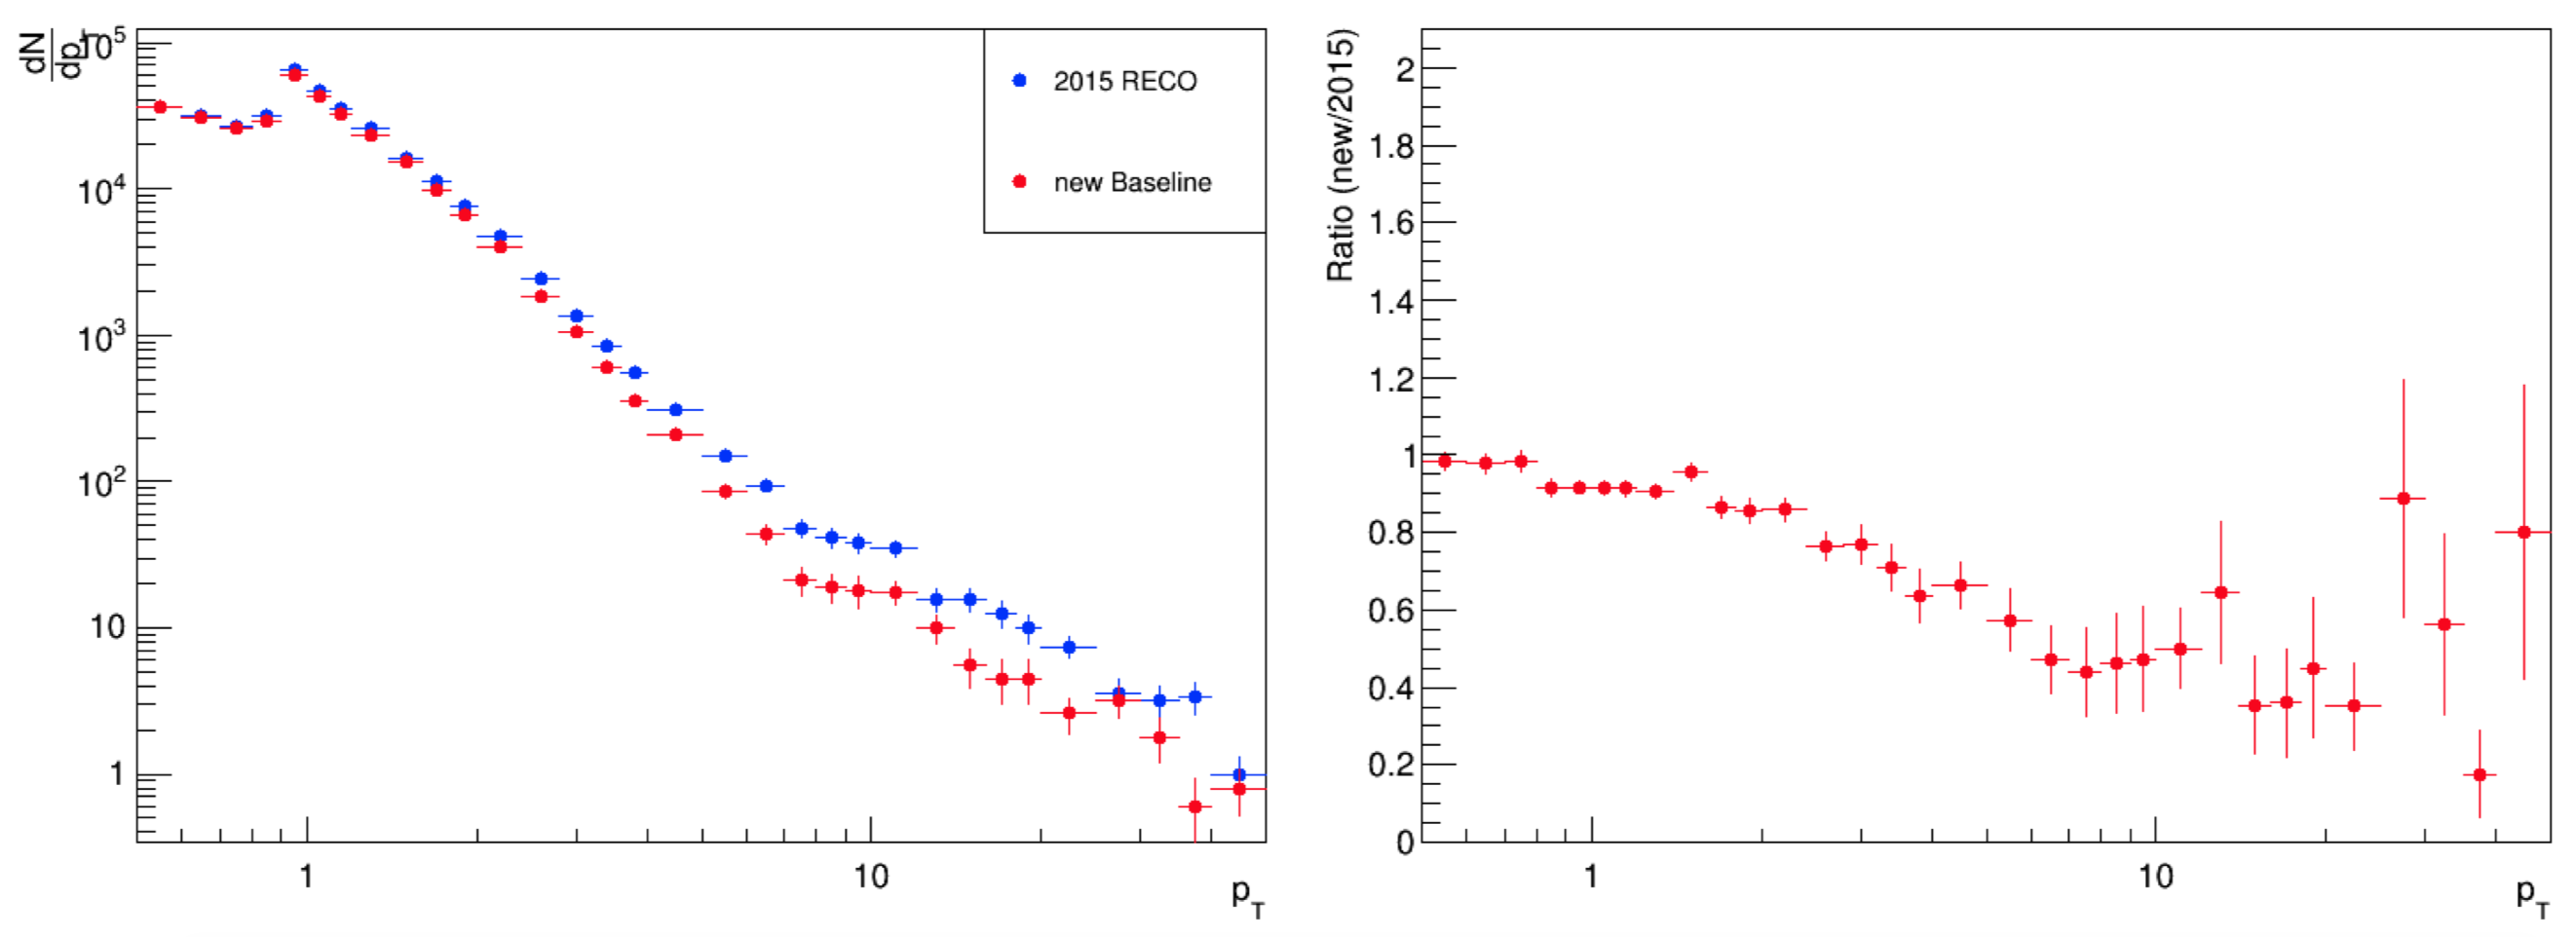
\includegraphics[width=.80\textwidth]{figures/DerivativeFollowerEfficiency.png}
\caption{}
\label{fig:stripDerivFollowerPerf}
\end{center}
\end{figure}


\subsubsection{Hybrid data format \label{subsubsec:hybridtracker}}
The Hybrid data format strategy is based on the principle that the standard FED zero suppression fails only for the fraction of APVs in which the baseline is either heavily shifted or distorted. When none of the two conditions are met, the Common Mode Noise calculated as a constant value to be subtracted to all the ADC of a single APV, is good enough for cluster findings. In fig. \ref{fig:stripBadAPV} it is shown the fraction of modules for which the full baseline needs to be reconstructed as function of centrality. 
For very central Pb-Pb collisions ~ 10 k APVs require a specific handling while for Minimum Bias events only ~100 APVs require a specific handling.

In this optic, it is possible to receive a significant data reduction to DAQ sending an hybrid data format containing the Virgin Raw data only for the APVs that require a special care. The APVs without pathology in the baseline are zero suppressed in the tracker FED using the standard zero suppression algorithm. In HLT, the tracker data will be unpacked and the standard HI Zero Suppression algorithm (Baseline Follower) is used to zero suppress the problematic APVs. 

The code needed to emulate the full chain is still being written so it is not yet available a precise measure of the actual data size in hybrid data format. However, a rough estimation indicates a factor 2 to 3 on the standard suppressed size. As a consequence, the goal of 30 kHz should be achieved.

    


 \begin{figure}[htbp]
\begin{center}
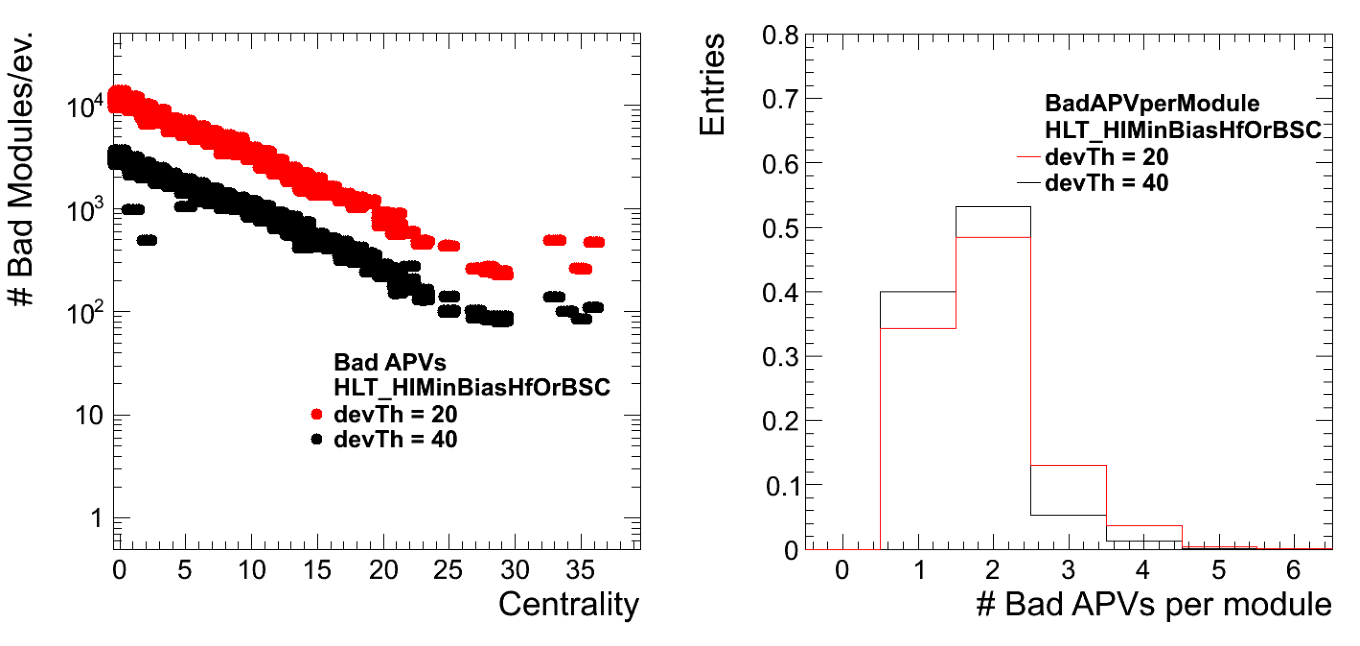
\includegraphics[width=.80\textwidth]{figures/BadAPV.pdf}
\caption{}
\label{fig:stripBadAPV}
\end{center}
\end{figure}
